\chapter{Theoretical background / applications}
\label{ch:applications}


\section{Graph Theory}
\label{sect:graph_theory}


\section{Areas of application}
\label{sect:app_areas}

	\subsection{Social networks}
	\label{ssect:social_networks}
	
	Social networks are today's natural candidates for graph based algorithms, as they have been rising to power and fame over the previous decade and a half. Of course most social graphs in use today are far too big for any client or server side application to handle, and are therefore only interesting to programmers and architects of database clusters, high performance grid-computing developers and data-center engineers. Because of this, I am going to confine myself to the topic of local sphere recommenders, where I believe small graph computing to be able to have some real world influence. In order to get to this point, we will first need to take a look at the shape and size of typical recommendation processes (themselves forming subgraphs of larger networks), which in the following section will be termed 'cascades'.
	
	
	\subsubsection{Network recommendation analysis}
	\label{sssect:net_rec_anal}
	
	\citet{RecCascades} have examined recommendation networks crystallizing from purchases based upon previously received product recommendations. In order to do this, they employed an online shopping system observing the product categories of DVDs, Music, Books and Videos (VHS). Users of that system were modelled as nodes in a graph, with the graph initially being completely unconnected. In this system people who bought a product (and only actual purchasers) were able to recommend the bought product to as many people  as they wanted via email; this resulted in a \textit{temporary} recommendation edge added between the two (user) nodes. This edge was then handled according to the following two criteria:
	
	\begin{enumerate}
		\item Recommendations received after a product was already bought by the receiving person were immediately deleted.
		\item Recommendations received which did not result in the product being bought (during the observational period) were also deleted.
	\end{enumerate}
	
	This procedure resulted not in a graph comprising all of the users and products bought throughout the system, but only a collection of - fragmented - subgraphs representing the recommendation cascades. The main question of the study then was to the size distribution of those cascades w.r.t. their count, and if properties of the original social network (e.g. density, degree distribution) had any influence on that distribution. 
	
	A second point of interest concerned the isomorphism classes of cascades, meaning their shape and size similarity. Therefore, a similarity measure had to be established, as the graph isomorphism problem is NP-hard and therefore impractical to use on a real-world study. This is why exact isomorphism matching was only used on cascades up to a graph size of 9 nodes; above that a graph \textit{signature} was computed including singular values (via SVD) of the graph adjacency matrix up to a size of 500 nodes. Above that, the signature only consisted of the number of nodes and edges as well as a histogram of in- and out-edges per node (degree distribution). The relation between cascade amount and size can be seen in Figure~\ref{fig:cascade_size_count} on page \pageref{fig:cascade_size_count}.

	The results of this study after a two-year period can be summarized as follows:
	
	\begin{itemize}
		\item The largest cascade (which also form connected components) accounted for less than 2.5\% of all nodes.
		\item Cascades did not only come in the form of trees (snowball effect) but form arbitrary graphs with splits, collisions as well as cycles.
		\item Splits are more common than collisions, however (as one would expect).
		\item The frequency of a cascade type (as computed by graph isomorphism) is not a strict monotonic function of cascade size, which points to the recommendation propagation process to be influenced by more subtle factors of the underlying social graph than just the network structure alone.
		\item Most cascades observed exhibited fewer than 9 nodes (with the exception of DVD recommendation cascades) and were of very small degree (just a little over 1 according to the visual representation found in the paper
	\end{itemize}
	
	\begin{figure}[ht]
		\begin{center}
			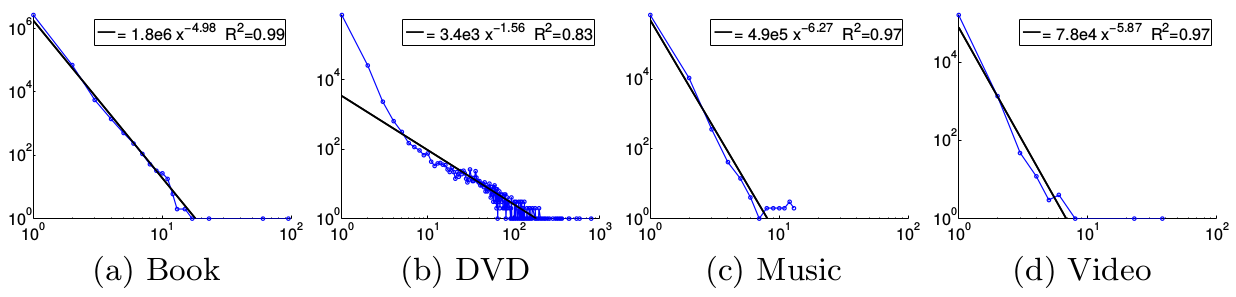
\includegraphics[width=1\textwidth]{figures/rec_cascades_size_count}
			\caption{Size distribution of recommendation cascades for four product categories}
			\small
			This diagram was taken from \citep{RecCascades}, page 7.
			\label{fig:cascade_size_count}
		\end{center}
	\end{figure}
	
	The above analysis holds several insights which in combination lead to a remarkable conclusion:
	
	\begin{enumerate}
		\item The cascades presented in the paper represent only 'successful' recommendations, i.e. the ones which receivers perceived as valuable enough to actually buy the product.
		\item The goal of any recommender algorithm (regardless on which item space it operates) is to produce exactly such valuable recommendations.
		\item Because most cascade sub-graphs were of very small size and degree, 'successful' recommendations can be assumed to originate from places in the direct neighborhood of a node.
	\end{enumerate}
	
	
	\subsubsection{The local sphere}
	\label{sssect:the_local_sphere}
	
	The concept of a local sphere and computations applied to it comes from the author's (possibly incorrect, but natural) insight that the relevance of recommendations behaves as a function of node vicinity:
	
	\begin{itemize}
		\item Lets call the whole social graph and all interactions in it the 'global sphere'.
		\item Recommendations to users are then computed over the global sphere, which takes an amount of resources exponential to the size of the underlying graph.
		\item Let's further assume that 95\% of all relevant (accepted) recommendations in a social network like facebook are those that are derived from the immediate local neighborhood of a node (less than 2 degrees, see section above..)
		\item This assumption is corroborated by the fact that two degrees are also what Facebook allows programmers (as of 2013) to query via their graph API from any authenticated user, apparently in an effort to prevent automatic traversal / exploration of their most valuable business asset.
		\item Let's call this immediate local neighborhood the 'local sphere'
	\end{itemize}
		
	Now let's also consider how modern publish/subscribe based frameworks (like Sails, Meteor, Hapi or Derby, only to mention some JavaScript libraries) handle data communication between server and client:
	
	\begin{itemize}
		\item The server offers some subscriptions on it's data, usually limiting access to items based on identity, authorization or user role provided by the client.
		\item The client defines some subscriptions on server-side data collections (tables), representing the client's wish for information regardless of it's status or authority.
		\item Publication as well as subscription can be seen as a mathematical subset of all the data in the database.
		\item An algorithm inside the respective framework resolves those (potentially conflicting) interests by computing the intersection set of the data provided / requested.
		\item The intersection data set is then pushed to the client (in our case the browser) as soon as it becomes available or is updated, which makes this model ideal for real-time interaction and communication between clients.
		\item The sum total of all the data pushed to the client is equivalent to the 'local sphere' we described earlier - HOWEVER - their inherent graph structure is lost during the transmission, so that the client can only see them as isolated fragments without context.
	\end{itemize}
	
	The combination of those two ideas now enables us to envision the following scenario:
	
	\begin{itemize}
		\item Instead of interpreting all data items in the local sphere as isolated entities, we retain their graph structure enabling the client to gain hitherto unachieved knowledge and insights into its already available data.
		\item We therefore need a graph library in the browser, not only to represent the local sphere graph, but also to analyze it in order to take intelligent actions that were previously reserved for the server-side (data center) infrastructure.
		\item No complex graph partitioning algorithm on the server is necessary, as we can use the natural set contraints inherent in any web application:
		\begin{itemize}
			\item e.g. in a social network, the client will have access to all its immediate friends, social activities and interest groups
			\item in a project management tool, the client naturally has access to the data of all team members, to-do lists, milestones, resources etc.
		\end{itemize}
		If our 95\%-relevance assumption mentioned earlier holds, we can achieve great scaling efficiency by introducing the local sphere concept:
		\begin{itemize}
			\item the client can immediately perform computations like recommendations on the subgraph of the local sphere.
			\item only recommendations accepted will have to be stored on the server (that is, cause additional network traffic).
			\item the client is easily able to recompute the relatively small local graphs in real-time, offering responsiveness far beyond today's best (server-side) infrastructures.
			\item as modern web frameworks transport all of the required data into the client store anyways, we do not add extra complexity to our servers and databases.
		\end{itemize}
		\item On the other hand, questions of data security / privacy will have to be dealt with, as we are talking about preemptively filling the client memory with possibly otherwise unnecessary or superfluous data.
	\end{itemize}
	
	
	\begin{figure}[ht]
		\label{fig_local_sphere}
		\begin{center}
			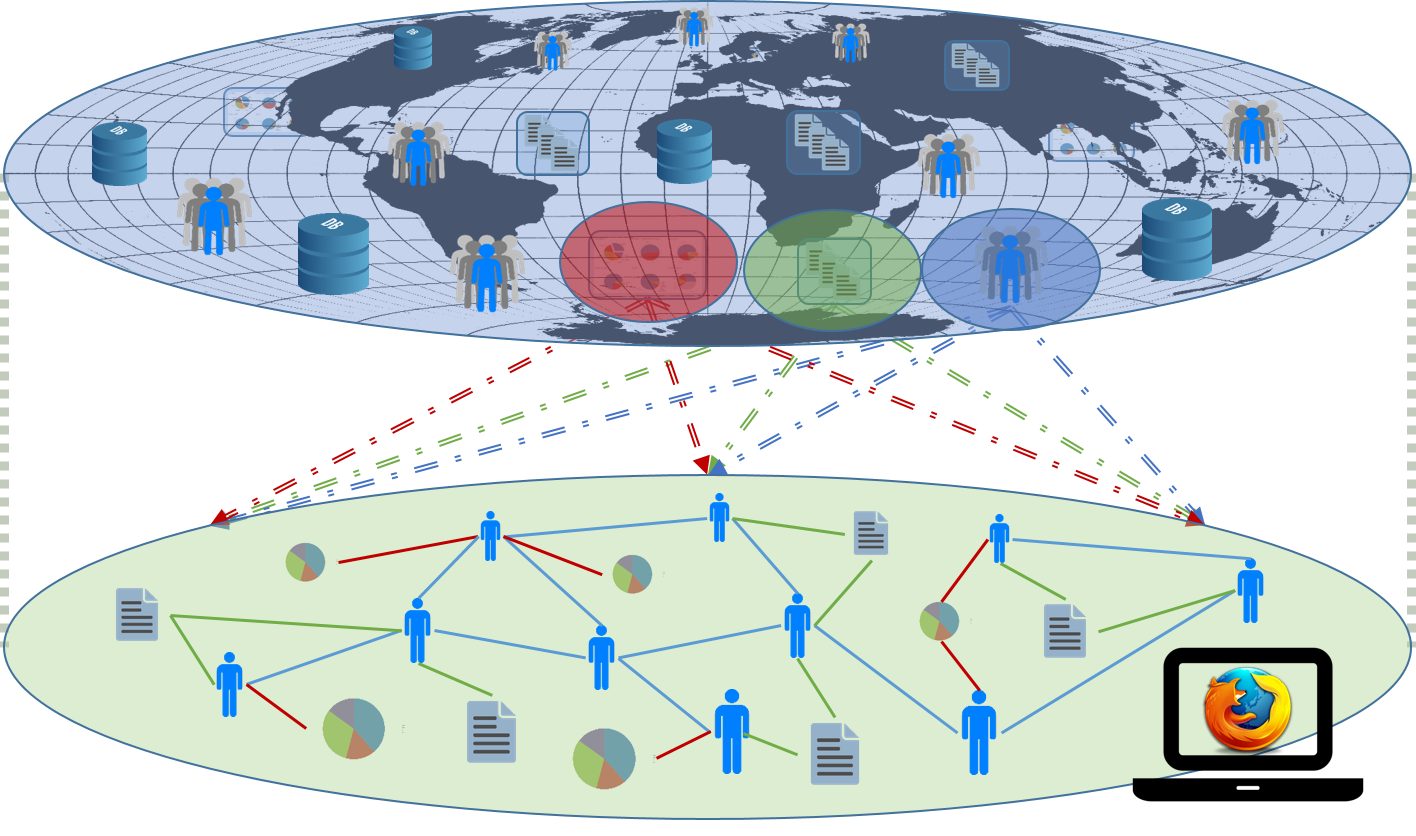
\includegraphics[width=1\textwidth]{figures/local_sphere}
			\caption{Local sphere projected from global sphere}
		\end{center}
		\small
		Only a very small portion of the global graph is actually visible from any connected client. The sum of all viewable items however, if properly conveyed to the client (i.e. with their connection information preserved), could form a subgraph of the whole network called the 'local sphere', which would allow the browser to utilize the underlying graph structure to extract hidden knowledge and perform graph computations on its own.
	\end{figure}
	
	
	Needless to say, GraphiniusJS would be an ideal candidate to explore this concept further and could, if used appropriately on carefully modeled local spheres, enable start-ups to compete with much larger companies employing complex and very expensive machine learning infrastructures.
	
	
	% \subsection{Communication networks}
	% \label{ssect:app_communication_networks}
	
	% \subsection{Transportation networks (Logistics)}
	% \label{ssect:app_transportation_networks}
	
	
	\subsection{Graph based image processing}
	\label{ssect:app_graph_img_proc}
	
	\begin{figure}[ht]
		\label{fig_graph_based_img_classification}
		\begin{center}
			
\includegraphics[width=1\textwidth]{figures/graph_img_class}
			\caption{Graph based image classification example}
		\end{center}
		\small
		1) a laser scan image of a nevus is oversegmented and 2) a graph extracted by interpreting region centroids as nodes and region adjacency as edges. 3) A belief propagation algorithm is applied to the resulting graph yielding 2) a converged state representing the nevus classification as benign or malignant.
	\end{figure}
	
	\subsection{Graph based NLP}
	\label{ssect:app_graph_nlp}
	
	\subsection{Biomedical applications (protein networks etc.)}
	\label{ssect:app_biomed}
	
	\subsection{Anonymization}
	\label{ssect:app_snonymization}
	
	\begin{figure}[ht]
		\label{fig_graph_based_img_classification}
		\begin{center}
			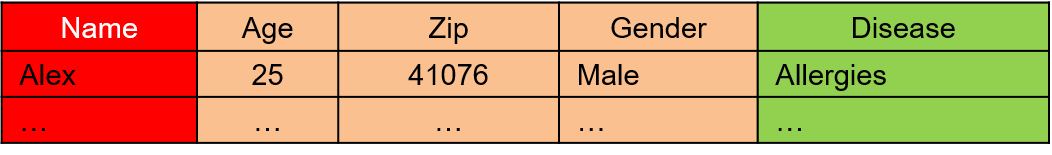
\includegraphics[width=0.9\textwidth]{figures/anonym/3typesofdata}
			\caption{The three types of data considered in (k-)anonymization}
		\end{center}
	\end{figure}
	
	
	\begin{figure}[H]
		\centering
		\begin{minipage}[b]{0.5\textwidth}
			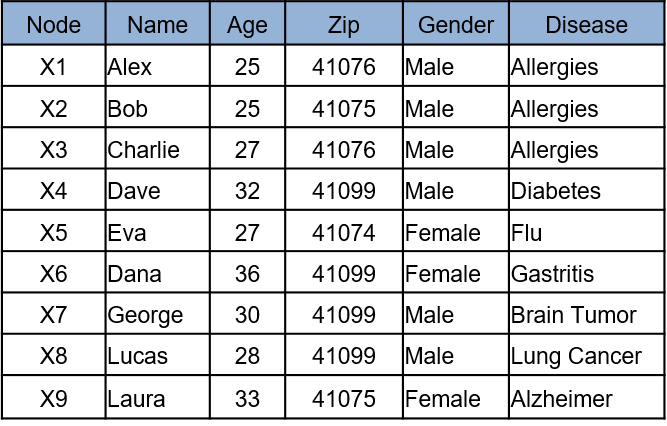
\includegraphics[width=\textwidth]{figures/anonym/k_anon_input}
		\end{minipage}
		\hfill
		\begin{minipage}[b]{0.418\textwidth}
			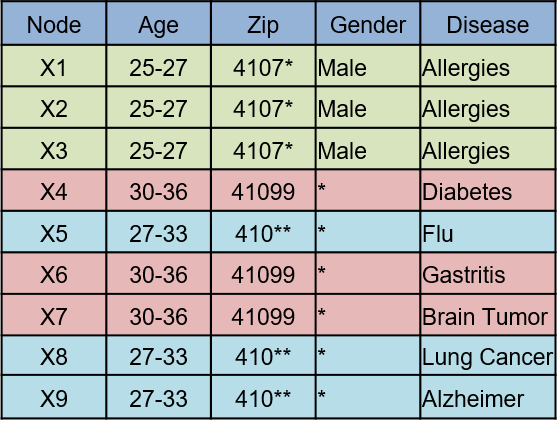
\includegraphics[width=\textwidth]{figures/anonym/k_anon_output}
		\end{minipage}
		\caption{Tabular anonymization: input table and anonymization result}
	\end{figure}	
	
	
	\subsection{Fraud detection}
	\label{ssect:fraud_detection}

	Polo chau's BP in MRF for spam classification work...

\section{Application specific requirements}
\label{section:app_requirements}

	\subsection{Data Structures}
	\label{ssect:data_gathering}
	
	\subsection{Data Cleaning}
	\label{ssect:data_cleaning}
	
	\subsection{Preprocessing}
	\label{ssect:preprocessing}
	
	Graph generation (ER model...)
	
	\subsection{Feature Selection}
	\label{ssect:feature_selection}
	
	\subsection{Data Mining}
	\label{ssect:data_mining}
	
	\subsection{Postprocessing}
	\label{ssect:postprocessing}
	
	\subsection{Visualization}
	\label{ssect:visualization}
	
	\subsection{Interaction / user feedback (iML)}
	\label{ssect:interaction}
	